\documentclass[12pt,twocolumn]{article}
\usepackage[margin=1.0cm]{geometry}
\usepackage{amsmath}
\usepackage{graphicx}
\usepackage{hyperref}
\title{Midterm 1 - PHYS180}
\author{Prof. Jordan C. Hanson}

\begin{document}
\maketitle
\small
\textbf{Part 1: Units 0-2.}
\begin{figure}
\centering
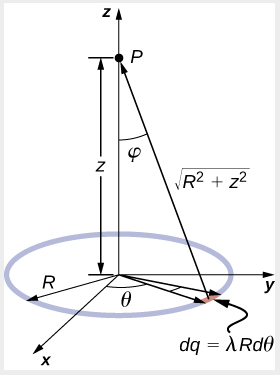
\includegraphics[width=0.2\textwidth]{ring.png}
\caption{\label{fig:ring} A ring of charge situated in the xy-plane.}
\end{figure}
\begin{figure}
\centering
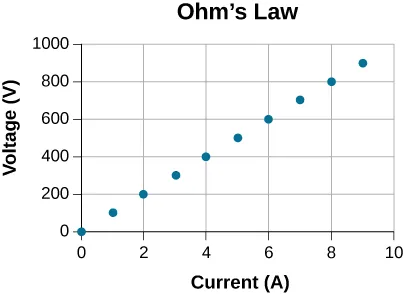
\includegraphics[width=0.33\textwidth]{Ohms.png}
\caption{\label{fig:circ} Voltage vs. current in a DC circuit.}
\end{figure}
\begin{enumerate}
\item Suppose we are charging a car battery with an average current of $I = \Delta Q/\Delta t = 2$ Amps, for 5 hours.  (a) How many Coulombs of charge did we put in the battery? (b) If a battery has 7 Amp hr of charge, for how long can it provide 0.5 Amps of current?
\item Consider Fig. \ref{fig:ring}.  A ring of charge $Q$ with radius $R$ is situated in the xy-plane.  (a) Show that if the function for $\vec{E}(z)$ is given by Eq. \ref{eq:eq1}, that it has the right \textit{units}. (b) Show that Eq. \ref{eq:eq1} has the correct \textit{limit} as $R \to 0$.
\begin{equation}
\vec{E}(z) = \frac{k Q z}{\left( z^2 + R^2 \right)^{3/2}} \hat{z} \label{eq:eq1}
\end{equation}
(c) Model the charged ring in xy-plane (\url{https://phet.colorado.edu/en/simulations/charges-and-fields}).  Plot the magnitude of the E-field as a function of inverse distance squared from the center, and show that the plot is linear for distances far from the center.  Draw your graph by hand and include it with your responses.
\item An evacuated tube uses an accelerating voltage of 40 kV to accelerate electrons to hit a copper plate and produce x-rays. What is the maximum speed of these electrons?
\item Show that units of V/m and N/C for electric field strength are indeed equivalent.
\item Imagine a capacitor that has the following properties: the distance between the plates is 1 mm, the voltage in the middle is 0 Volts, $V_{\rm max} = 6$ Volts, $V_{\rm min} = -6$ Volts, and $\Delta V = 12$ V.  (a) What is the electric field in between the plates? (b) If an electron is accelerated by the capacitor voltage, what is the kinetic energy in eV? (c) Create a similar capacitor in our modeling software (\url{https://phet.colorado.edu/en/simulations/charges-and-fields}) that has a 240 V potential difference between the plates, and graph the voltage as a function of position between the plates.  Show that the slope of voltage is equal to the E-field.  Draw your graph by hand and include it with your responses.
\item (a) Suppose we allow 5 mA of current to flow onto a capacitor for 5 seconds.  How much charge is stored in the capacitor? (b) After 5 seconds, the capacitor voltage is measured to be 5.0 V.  What is the capacitance? (c) If this capacitor is filled with Teflon, what will the new capacitance be? (d) Now assume four such capacitors are connected in parallel.  What is the total capacitance?
\item Consider Fig. \ref{fig:circ}.  (a) What is the resistance of the circuit? (b) Suppose the data, including statistical errors, was given by Tab. \ref{tab:1}.  Compute the reduced $\chi^2$ statistic, given the model assumed from part (a).
\begin{table}
\centering
\begin{tabular}{| c | c | c |}
\hline
\textbf{Current} & \textbf{Voltage} & \textbf{Err. in Voltage} \\
0 & 5 & 5 \\
1 & 95 & 5 \\
2 & 204 & 5 \\
3 & 310 & 5 \\
4 & 395 & 5 \\
5 & 520 & 5 \\
6 & 600 & 5 \\
7 & 705 & 5 \\
8 & 795 & 5 \\
9 & 910 & 5\\
\hline
\end{tabular}
\caption{\label{tab:1} The actual data from Fig. \ref{fig:circ}.}
\end{table}
\item (a) Find the voltage drop in an extension cord having a 0.0600 $\Omega$ resistance and through which 5.00 A is flowing. (b) A cheaper cord utilizes thinner wire and has a resistance of 0.300 $\Omega$. What is the voltage drop in it when 5.00 A flows? (c) Why is the voltage to whatever appliance is being used reduced by this amount? What is the effect on the appliance?
\item Consider Fig. \ref{fig:series}.  The values of each resistor are quoted in Tab. \ref{tab:2}, along with associated errors.  What is the total resistance, with its associated error?
\begin{figure}
\centering
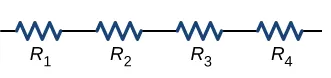
\includegraphics[width=0.35\textwidth]{fourSeries.png}
\caption{\label{fig:series} Four resistors in series.}
\end{figure}
\begin{table}
\centering
\begin{tabular}{| c | c | c |}
\hline
\textbf{Resistor} & \textbf{Resistance} & \textbf{Error} \\
$R_1$ & 1.00 k$\Omega$ & 50 $\Omega$ \\
$R_1$ & 0.95 k$\Omega$ & 50 $\Omega$ \\
$R_1$ & 1.05 k$\Omega$ & 50 $\Omega$ \\
$R_1$ & 0.95 k$\Omega$ & 50 $\Omega$ \\
\hline
\end{tabular}
\caption{\label{tab:2} The resistances, with associated errors, for the resistors in Fig. \ref{fig:series}.}
\end{table}
\item (a) Verify that the units of a volt-ampere are watts, as implied by the equation $P=IV$. (b) Show that the units V$^2/\Omega=1$ W, as implied by the equation $P = V^2/R$. (c) Show that the units A$^2 \Omega=1$ W, as implied by the equation $P = I^2 R$.
\item Verify the energy unit equivalence that 1 kW hr $= 3.60\times 10^6$ J.
\item An electric water heater consumes 5.00 kW for 2.00 h per day. What is the cost of running it for one year if electricity costs 12.0 cents per kiloWatt hour?
\item Using our DC circuit modeling software (\url{https://phet.colorado.edu/en/simulations/circuit-construction-kit-dc}), create a DC circuit that consumes 100 W, split across four devices (25 W each).  Install switches such that each device can be turned on or off independently from the others.  List the total current from the battery for each combination of switches.  Draw your circuit design by hand, and list the results by your design.
\item Consider Fig. \ref{fig:complex}.  Let $V_1 = 12$ V, $V_2 = 1.2$ V, and all resistors have a value of $2$ k$\Omega$. (a) Solve for all currents through all resistors.  (b) Confirm your results in our DC circuit simulator.
\item (a) Design an RC circuit with an RC time of 1 second.  (b) Suppose the charging EMF is 5 V.  Let $t=0$ correspond to when current begins to flow.  When does the capacitor voltage reach 2.5 V? (c) Confirm this with the AC circuit simulation tool (\url{https://phet.colorado.edu/en/simulations/circuit-construction-kit-ac}).
\item Consider Fig. \ref{fig:complex2}. Suppose each AA battery has an EMF of 1.5 V and an internal resistance of 0.1 $\Omega$, and the load resistance $R$ is 5 $\Omega$.  (a) What current flows through $R$? (b) What is the power consumption in $R$? (c) If the AA batteries each have 2000 mA hr of charge, how long before they drain?
\end{enumerate}
\begin{figure}
\centering
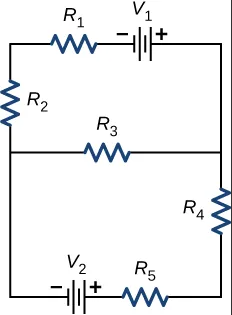
\includegraphics[width=0.175\textwidth,trim=0cm 0cm 0.1cm 0.0cm,clip=true]{kirchhoff_3.png}\caption{\label{fig:complex} A circuit with batteries and resistors.}
\end{figure}
\begin{figure}
\centering
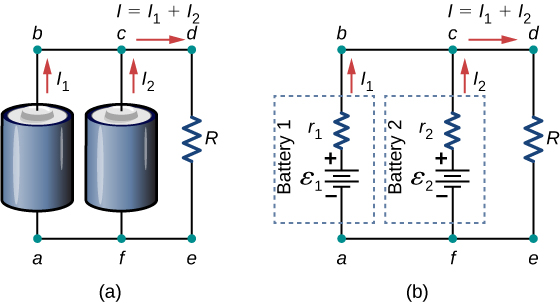
\includegraphics[width=0.35\textwidth]{parallel_batt.jpg}
\caption{\label{fig:complex2} (a) Two AA batteries connected in parallel. (b) Circuit diagram for the situation.}
\end{figure}
\clearpage
\textbf{Part 2. Units 2-3.}
\begin{figure}
\centering
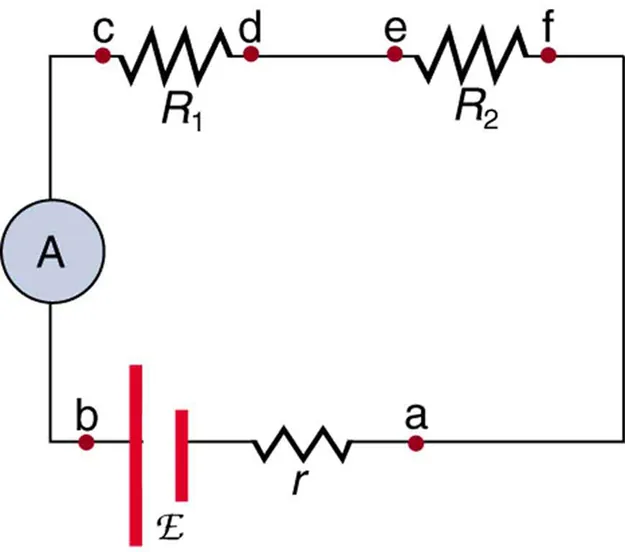
\includegraphics[width=0.2\textwidth]{ammeter.png} \hspace{0.2cm}
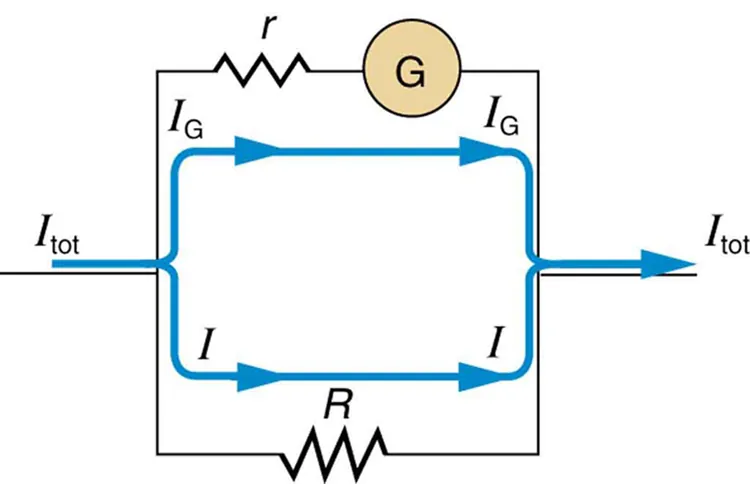
\includegraphics[width=0.25\textwidth]{galvo_2.png}
\caption{\label{fig:ammeter} (Left) An ammeter in series with $R_1$ and $R_2$, and a battery with emf $\mathcal{E}$ and internal resistance $r_b$. (Right) The internal structure of the ammeter, with galvanometer G, internal resistance $r$ and shunt resistance $R$.}
\end{figure}
\begin{figure}
\centering
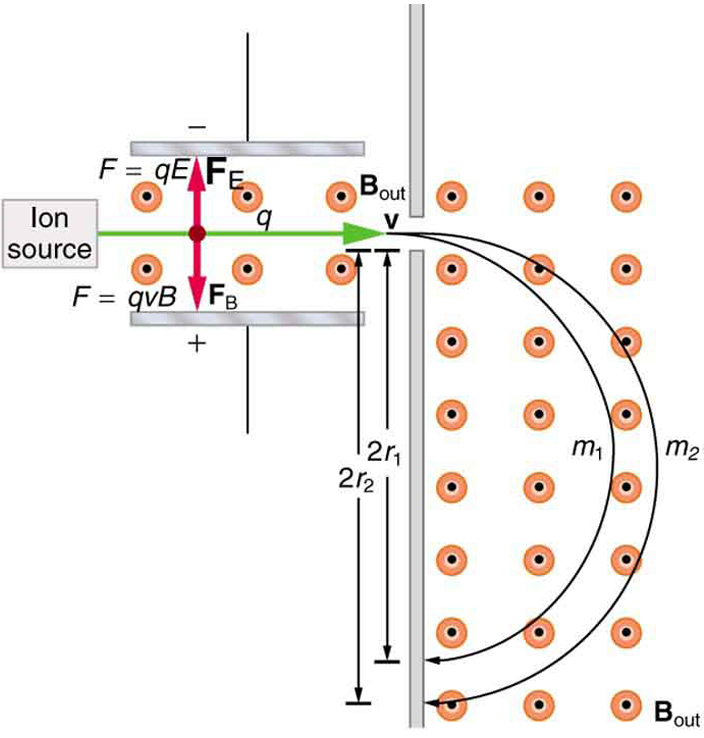
\includegraphics[width=0.35\textwidth]{mass_spec.jpeg}
\caption{\label{fig:mass} The basic structure of a mass spectrometer.}
\end{figure}
\begin{enumerate}
\item Suppose the ammeter in Fig. \ref{fig:ammeter} has an internal resistance $r = 10\Omega$, and a ``shunt'' resistance of $R = 0.1\Omega$.  The circuit has $R_1 = 1$ k$\Omega$, $R_2 = 1$ k$\Omega$, $\mathcal{E} = 12$V and $r_b = 1 \Omega$. (a) Calculate the total resistance of the ammeter, $R_{\rm A}$. (b) Calculate the total current flow from the battery, $I_{\rm total}$. (c) What is the decrease in voltage across the ammeter? (d) What is the current flow to G, the galvanometer, $I_{\rm G}$?
\item Consider Fig. \ref{fig:mass}.  (a) Show that if $F_B = F_E$, that the velocity of the positive ions must be $v = E/B$.  (b) For the section after the capacitor, set the centripetal force equal to the Lorentz force to derive an expression for the radii $r_1$ and $r_2$. (c) Suppose we know that $r_1 = 25$ cm, and corresponds to hydrogen ions.  What is $r_2$, if those ions are heliums with +1 charge (missing one electron)? \\
\item Consider Fig. \ref{fig:tok}, in which a \textit{tokamak} is shown.  In your own words, explain why the plasma in this fusion reactor is contained within the toroidal volume.
\end{enumerate}
\begin{figure}
\centering
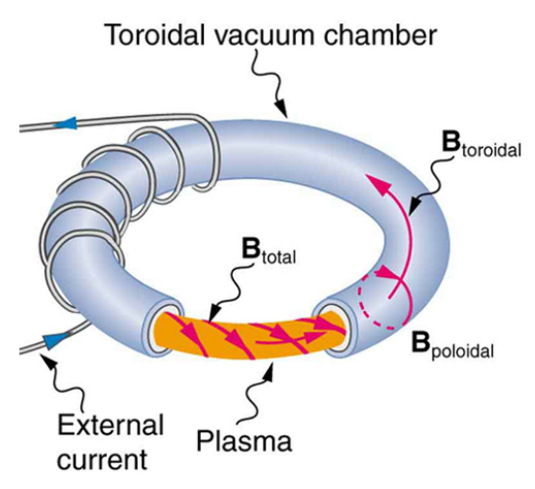
\includegraphics[width=0.35\textwidth]{tokamak.png}
\caption{\label{fig:tok} This structure is called a \textit{tokamak}, and it is used to confine plasma in a fusion reactor.}
\end{figure}
\end{document}